\documentclass{article}


% if you need to pass options to natbib, use, e.g.:
%     \PassOptionsToPackage{numbers, compress}{natbib}
% before loading neurips_2023


% ready for submission
\usepackage[final]{cs152}



\usepackage[utf8]{inputenc} % allow utf-8 input
\usepackage[T1]{fontenc}    % use 8-bit T1 fonts
\usepackage{hyperref}       % hyperlinks
\usepackage{url}            % simple URL typesetting
\usepackage{booktabs}       % professional-quality tables
\usepackage{amsfonts}       % blackboard math symbols
\usepackage{nicefrac}       % compact symbols for 1/2, etc.
\usepackage{microtype}      % microtypography
\usepackage{xcolor}         % colors
\usepackage{graphicx}       % images
\usepackage{float}          % for the [H] option
\usepackage{hyperref}


\title{YOLOv1 Object Detection Model}


% The \author macro works with any number of authors. There are two commands
% used to separate the names and addresses of multiple authors: \And and \AND.
%
% Using \And between authors leaves it to LaTeX to determine where to break the
% lines. Using \AND forces a line break at that point. So, if LaTeX puts 3 of 4
% authors names on the first line, and the last on the second line, try using
% \AND instead of \And before the third author name.


\author{%
  Isaac Chung \\
  Harvey Mudd College \\
  \texttt{ischung@g.hmc.edu} \\
  \And
  Brian Cha \\
  Harvey Mudd College \\
  \texttt{brcha@g.hmc.edu} \\
  \And
  Erin Li \\
  Harvey Mudd College \\
  \texttt{erli@g.hmc.edu} \\
  \And
  Patrick Liu \\
  Harvey Mudd College \\
  \texttt{hualiu@g.hmc.edu} \\
}


\begin{document}


\maketitle


\begin{abstract}
  For our final project, our goal is to implement a YOLOv1 (You Only Look Once) Object Detection model. We chose to implement YOLO because we thought it would be interesting to see how a model can analyze images and videos in real-time while achieving reasonable performance. This project also correlates to the topics we learned in Professor Wloka's Lab for Cognition and Attention in Time and Space, which primarily focuses on computer vision, spatial disparities, and depth perception in an immersive research setting. Our approach is to develop multiple object classes, 20 to be exact, and implement YOLO's unique architecture to achieve high performance predictions in a single pass. As the original paper suggested, we used the PASCAL VOC dataset, which constituted around 5 gigabytes, to train our model, and we further tested the model's predictions using our own input images. The results showed reasonable training and validation performance, indicating that our model sufficiently predicts objects but there is definitely room for improvement. We hope to demonstrate the effectiveness of our YOLOv1 model through its potential applications in real-world computer vision tasks.
\end{abstract}


\section{Introduction and related work}

Object detection is a fundamental task in computer vision. In fact, object detection can be applied to a plethora of computer vision scenarios such as in autonomous vehicle systems to augmented reality. It is important to note that object detection is quite different from object recognition since it is designed not only to recognize objects but also to determine their relative positions within the image, which we visualize using bounding boxes. What makes YOLO very interesting is that it is much faster than previous object detection algorithms and is capable of real-time object detection in an efficient manner. This is possible by applying a single forward pass to the entire image and predicting where the bounding boxes are positioned within the image as well as the class probabilities. Previous object detection algorithms rely on networks that scan regions of the image, which take multiple stages of visual processing. \\

Our primary resource for creating our YOLO model comes from the original paper: ``You Only Look Once: Unified, Real-Time Object Detection'' by Joseph Redmon. However, we also derived our ideas from various Youtube tutorials and explanations that are cited below. We dove deep into the research papers that our original paper got inspiration from, which highlighted important object detection fundamentals such as convolutional activation for visual recognition, scalability, and deep learning applications. \\

Our work will build upon these diverse perspectives of object detection by implementing the original YOLOv1 algorithm. Our goal is to see how Joseph Redmon was able to develop this model and explore its capacity to detect objects in image and video mediums, particularly assessing its performance with its intricate loss function. By becoming more familiar with YOLO principles, we hope to understand how YOLO has stood out as a revolutionary framework in the computer vision space, and how we can further improve our model to apply it to more complex, dynamic settings.

\section{Datasets}
The data that we used to train our YOLOv1 model is called the PascalVOC dataset, consisting of 2007-2012 images. The data was downloaded from Kaggle, and the link to this dataset is provided below. Within this dataset, there is a directory that specifies the images themselves and the labels. Each image has a number associated with it; for example, an image named 00001.jpg has a corresponding .txt file in the labels directory called 00001.txt. The image directory only contains .jpg files, containing one or more of the 20 predefined classes. Each of the 20 classes are listed here: \\

Person: person. \\
Animal: bird, cat, cow, dog, horse, sheep. \\
Vehicle: airplane, bicycle, boat, bus, car, motorbike, train. \\
Indoor: bottle, chair, dining table, potted plant, sofa, tv (or monitor). \\

We can also provide an example of such an image to label pairing: \\

The following image is classified as 00001.jpg. \\

\begin{figure}[H]
  \centering
  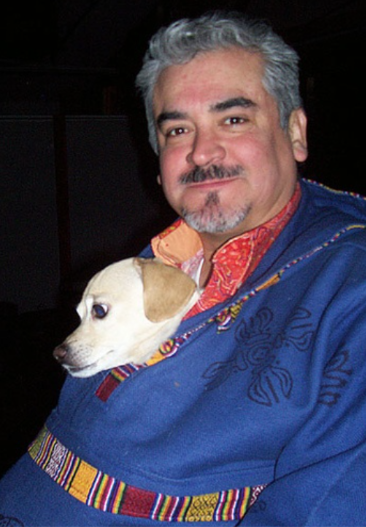
\includegraphics[width=0.4\textwidth]{Images/man_dog.png}
  \caption{Image 00001.jpg. It depicts a man and a dog}
  \label{fig:example}
\end{figure}

Here is the corresponding 00001.txt. \\

\texttt{11 0.34419263456090654 0.611 0.4164305949008499 0.262 \\
14 0.509915014164306 0.51 0.9745042492917847 0.972} \\

We can also specify which ids each class of object corresponds to: \\

0. Airplane 	1. Bicycle 	2. Bird 	3. Boat 	4. Bottle 	5. Bus		6. Car

7. Cat 		8. Chair 	9. Cow 	10. Dining Table 	11. Dog 	12. Horse 	13. Motorbike 	

14. Person	15. Plant 	16. Sheep 	17. Sofa 	18. Train 	19. TV \\

Using the label above, the first number represents the class id. Hence, 11 represents the dog class and 14 represents the person class. The next two numbers represent the midpoint of the object, defined as x and y, relative to the entire image. Hence, (0, 0) would indicate the top left corner of the image and (1, 1) would represent the bottom right corner. \\

Since a person takes up most of the image, it's no surprise that its midpoint is positioned around the center of the entire image. Meanwhile, the dog is closer to the bottom left quadrant of the image, so it is reasonable that its midpoint is sanctioned in the bottom left quadrant. \\

The two values that follow represent the length of the width and height of a particular object of interest in the form of a rectangle. Since these coordinates are relative to the entire image, it is important to note that a value of 1 would represent the entire width or height of the image. The man embodies most of the image, so the rectangle representing him would be very large. The dog is much smaller than the man, so its rectangle would also be smaller, which is highlighted by its width and height measurements. \\

Lastly, we would like to mention that we chose to utilize the PascalVOC dataset over all other available datasets online because we wanted to reproduce the results from the original paper. The model from the paper used the PascalVOC dataset for training, and we wanted to compare results throughout the stages of our implementation to see if we were on the right track. However, we would also like to point out that the original paper only used the PascalVOC dataset for 2007 and 2012. For us, we utilized the datasets from 2007-2012 because we wished to train our model on more data, especially since we have much more computing power than in 2016 when this process was not even feasible. \\

Here are some summary statistics for our labels in the data: \\

Total number of images: 43,233 images

Total number of objects in images: 52,090 labels

Labels for each class: \\
Class 0: 1456 occurrences \\
Class 1: 1401 occurrences \\
Class 2: 2064 occurrences \\
Class 3: 1403 occurrences \\
Class 4: 2233 occurrences \\
Class 5: 1035 occurrences \\
Class 6: 4468 occurrences \\
Class 7: 1951 occurrences \\
Class 8: 3908 occurrences \\
Class 9: 1091 occurrences \\
Class 10: 1030 occurrences \\
Class 11: 2514 occurrences \\
Class 12: 1420 occurrences \\
Class 13: 1377 occurrences \\
Class 14: 17784 occurrences \\
Class 15: 1967 occurrences \\
Class 16: 1312 occurrences \\
Class 17: 1053 occurrences \\
Class 18: 1207 occurrences \\
Class 19: 1416 occurrences \\


\section{Methods}

The overarching goal of our YOLOv1 model is to classify and locate objects in an image or video using bounding boxes for visualization. Future versions of YOLO incorporate other features such as anchor boxes, but we will not dive into these unique features since they are absent in our version of YOLO. \\

Our algorithm starts off by splitting an input image into SxS grids. We followed the original paper's default value of 7. Here is an example of such an image:

\begin{figure}[H]
  \centering
  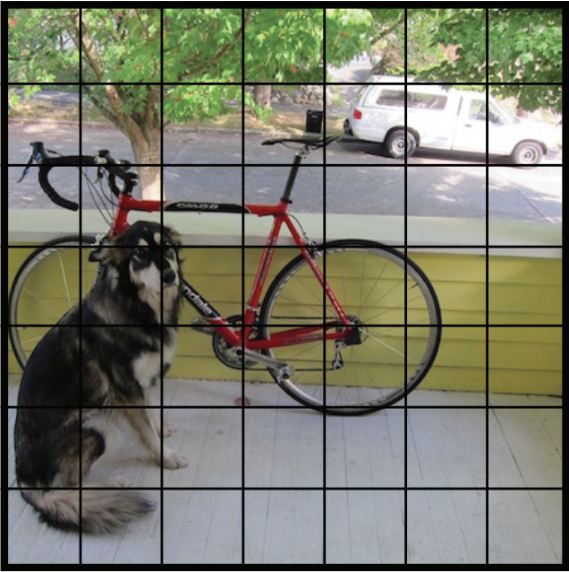
\includegraphics[width=0.4\textwidth]{Images/Grid.png}
  \caption{Example input image, with an \(7 \times 7\) grid overlay}
  \label{fig:example}
\end{figure}

From this image, we can clearly see a dog, a bike, and a car, each of which takes up more than one cell. It would be redundant to have each cell that contains a part of an object to detect the whole object; for example, it would take repeated work for each cell that contains the dog to detect the dog for that cell. Hence, we will refactor each cell so that the cell containing an object's midpoint is responsible for detecting that object in the entire image. We can modify our image to help visualize this function:

\begin{figure}[H]
  \centering
  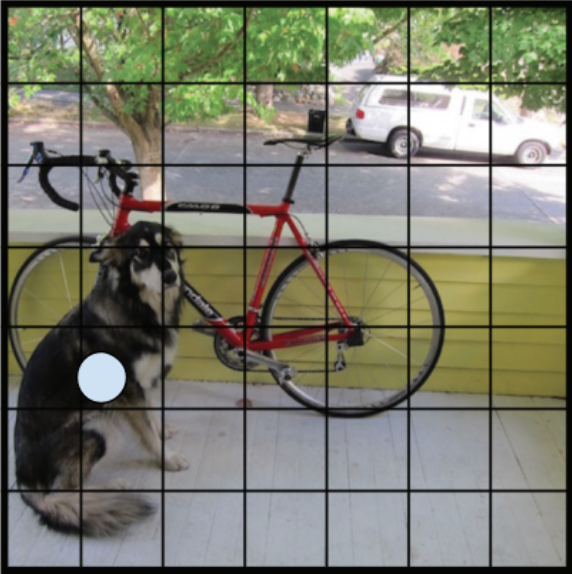
\includegraphics[width=0.4\textwidth]{Images/Grid_dot.png}
  \caption{Midpoint dot for dog drawn as light blue circle}
  \label{fig:example}
\end{figure}

Hence, the cell represented by (4, 1) or the 5th row and 2nd column will be responsible for detecting the dog. \\

Each cell in the SxS grid will predict B bounding boxes, and these predictions will not be limited by the size of the cells. In other words, the bounding boxes are valid if they contain at least one corresponding cell that they are a part of. An example of this can be shown here:

\begin{figure}[H]
  \centering
  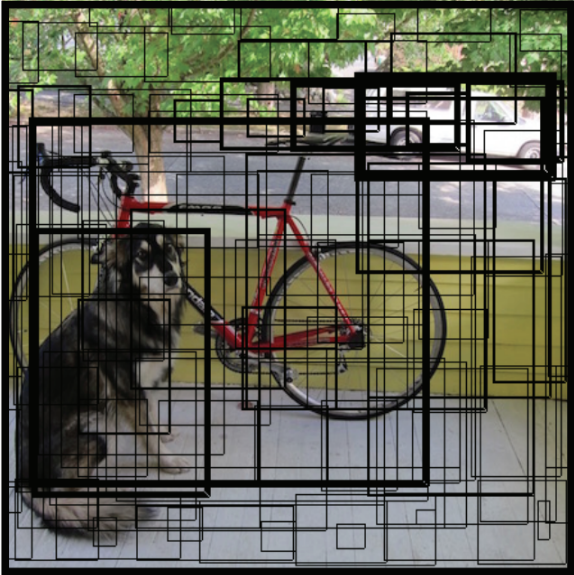
\includegraphics[width=0.4\textwidth]{Images/Grid_bbox.png}
  \caption{All bbox predictions drawn. Thicker bboxes indicate higher IOU}
  \label{fig:example}
\end{figure}

This looks quite messy, but it makes sense why. Many of the cells contain no objects, but they are still predicting bounding boxes. Hence, we may end up with many random bounding boxes as shown above. To make sure to choose the bounding boxes that contain objects of interest, we select the bounding boxes that have a high confidence score from our model. Our confidence score is determined by the Intersection over Union (IoU) metric between the predicted box and the ground truth. Hence, we can see that the bounding boxes around the dog, bike, and car have thicker lines because they have significantly higher IoU scores than the others, primarily because these predicted bounding boxes contain many actual bounding boxes provided by the labels. \\

By filtering out the undesired bounding boxes, we are left with this image:

\begin{figure}[H]
  \centering
  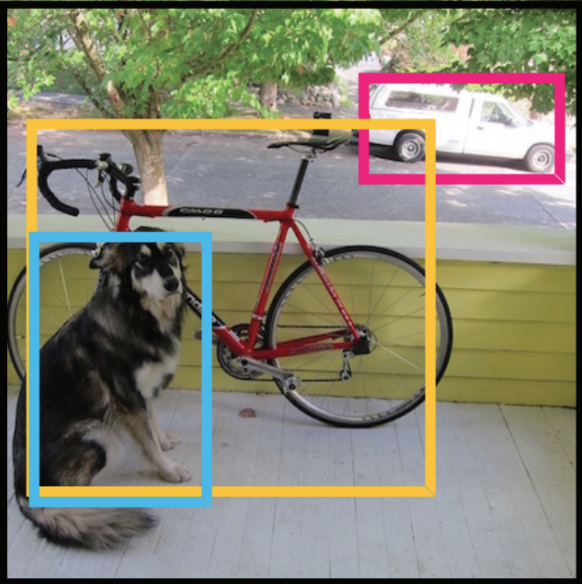
\includegraphics[width=0.4\textwidth]{Images/Grid_detections.png}
  \caption{Bboxes that contain objects}
  \label{fig:example}
\end{figure}

We have our bounding boxes around our objects of interest, but there must be a way to classify each bounding box to its corresponding object classes. Therefore, each cell in the SxS grid predicts a class probability as well. An example of this is shown here:

\begin{figure}[H]
  \centering
  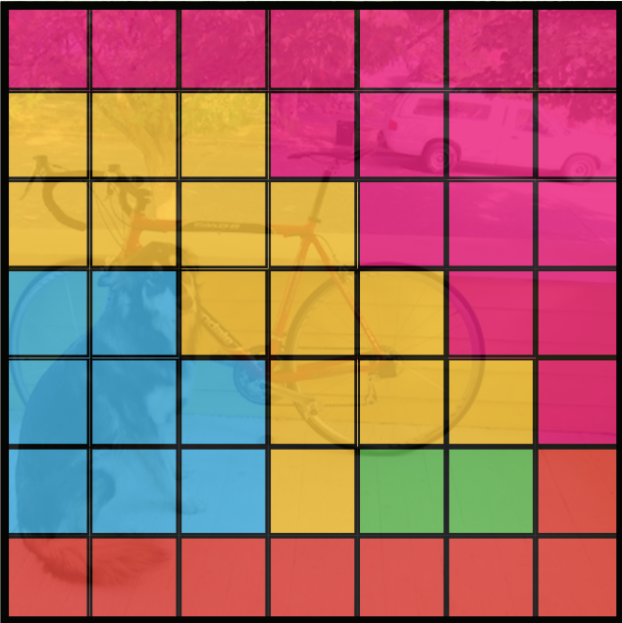
\includegraphics[width=0.4\textwidth]{Images/Grid_class.png}
  \caption{Class probabilities for each cell. Blue represents a dog, yellow represents a bike, magenta represents a car, and red represents a dining table}
  \label{fig:example}
\end{figure}

It is easy to distinguish between colors, so we had each color represent a particular class. In this case, blue represents a dog, yellow represents a bike, magenta represents a car, and red represents a dining table. Using these classifications, the class probabilities and bounding boxes are internally matched up together such that each bounding box is labeled with the correct class. \\

It is important to express how we assess the performance of our YOLOv1 model. Particularly, we want to evaluate how correct or incorrect our model is in terms of the loss. Here is a visual representation of the mathematics behind our loss function as described in the original paper:

\begin{figure}[H]
  \centering
  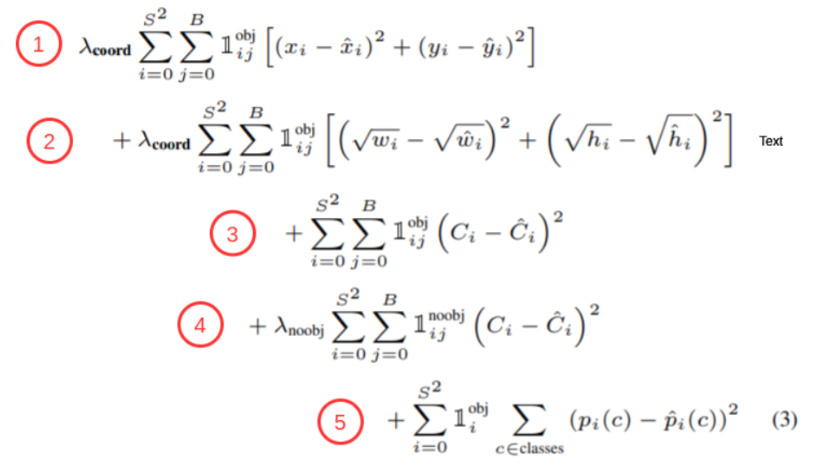
\includegraphics[width=0.8\textwidth]{Images/loss.png}
  \caption{YOLOv1 loss function}
  \label{fig:example}
\end{figure}

Before we dive into the specifics, we would like to explain what $1_{ij}^{obj}$ is and its purpose. $1_{ij}^{obj}$ is a measurement of how well a particular bounding box matches with a truth class. $i$ represents a cell and $j$ represents the $j$th bounding box in cell $i$. Hence, $1_{ij}^{obj}$ evaluates to $1$ if the $j$th bounding box of cell $i$ matches with a class and 0 otherwise. Intuitively, $1_{ij}^{noobj}$ is the exact opposite of $1_{ij}^{obj}$. \\

Now, we would like to analyze the loss function by breaking it up into parts as shown: \\

1. We first loop over every cell in the SxS grid and every bounding box in each cell. If the bounding box matches with a class, the loss function will minimize the error between the predicted bounding box's midpoint and the true bounding box's midpoint. In summary, we are minimizing the squared error.

2. We want to loop over every cell in the SxS grid and through each bounding box. Hence, if the bounding box matches with a class, the loss function will minimize the error between the width and height of the predicted and true bounding boxes.

3. Again, we loop over every grid cell and bounding box, but this time, we minimize the error between the confidence of the predicted and true bounding boxes.

4. We loop over every grid cell and bounding box, and if the bounding box does not match with any class, we minimize the error between the confidence of the predicted bounding box and 0, indicating no object found.

5. Lastly, we loop over all grid cells. If at least one bounding box in that cell matches with a particular class, we minimize the errors between the predicted and true class probabilities for all classes available.

6. We repeat this process for every iteration in our algorithm. \\

The hyperparameters utilized for our model were derived from the original paper. Here is a list of the hyperparameters used to train our model: \\

1. Seed = 123; a fixed seed is necessary for reproducibility. 		

2. Learning Rate = 2e-5 	

3. Batch Size = 16 			

4. Weight Decay = 0 		

5. Epochs = 1000		

6. Number of Workers = 2 		

7. Pin Memory = True

\section{Results and experiments}
Here is a plot representing the performance of our model on our training dataset. 

\begin{figure}[H]
  \centering
  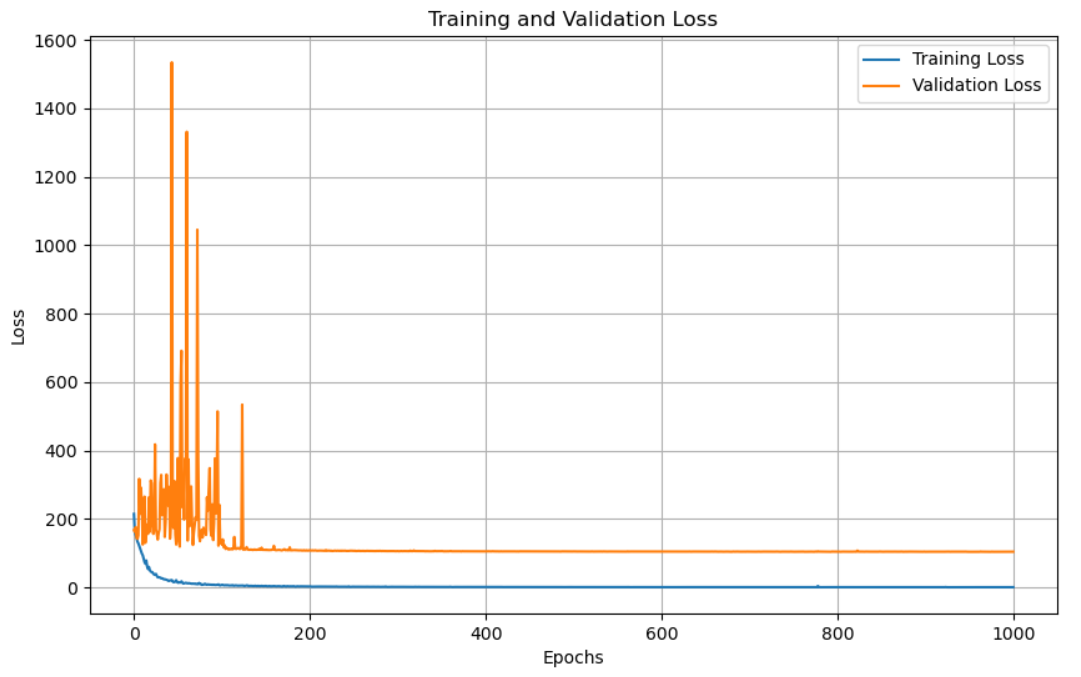
\includegraphics[width=0.8\textwidth]{Images/train_val.png}
  \caption{Our training and validation loss}
  \label{fig:example}
\end{figure}

As shown, our validation loss is much higher than our training loss, indicating that our model tends to overfit on the data. Unfortunately, we lack the time to implement a regularization feature to minimize the validation loss, especially since our loss function is already highly complex.


\section{Conclusion and future work}
Throughout our experimentation, our YOLOv1 model highlighted several key insights. Firstly, the model displayed reasonable performance in real-time object detection tasks, evoking a balance between speed and accuracy. We utilized evaluation metrics such as precision, recall, and mAP, otherwise known as the mean average precision, to assess the model's ability to detect objects across diverse classes. This prompts users to carefully consider this particular balance based on their specific application requirements. The diversity and complexity of the dataset also proved to be important in evaluating the model's performance. Exposing our model to a diverse range of images allowed it to learn more complex trends than it would with similar images. We also saw that tuning model parameters, such as adjusting bounding box size and the IOU metrics, helped us optimize our model. Overall, we would recommend that the users use our results with a deep consideration for dataset diversity, careful analysis of the speed-accuracy trade-offs, and experimentation with hyperparameters. \\

For the future, we can extend our project to involve testing the model on new datasets, particularly with video data and the COCO dataset. We can also explore modifications to the YOLOv1 architecture for improved accuracy across image-video domains and investigate its adaptability to address different computer vision challenges beyond object detection, such as image segmentation and pose estimation. Diving into these different paths could contribute to the continuous evolution and application of our YOLOv1 model across different computational fields.


\section{Broader impacts}
Our YOLOv1 model has been utilized for a plethora of positive and negative applications. On the positive side, our model enhances state-of-the-art object detection algorithms, including autonomous vehicle systems, surveillance processing, and medical imaging. The most impressive feature of our model that encapsulates these applications is its ability to provide real-time, accurate object detection. Hence, we believe that this model has the potential to improve safety, efficiency, and decision-making processes across a spectrum of computer vision domains. \\

On the other hand, there are ethical considerations associated with our model. It is important to note that the training data has been developed by humans; thus, it is inevitable that human biases exist within our data. The model's performance can be assessed based on the data it is trained on. Hence, the model's predictions may be swayed by the biases that are inherently present in the training data, and we must ensure to mitigate the effect of these biases to get accurate, reliable results. Additionally, YOLO is susceptible to unethical use, especially in terms of privacy. YOLO can be utilized in military applications and surveillance cameras that have the potential to leak private information and get visual data of an individual without their consent. There must be a balance between technological advancements and privacy safeguards to prevent the misuse of object detection models that incorporate YOLO systems. \\

We would also like to note that our training process took a couple of days to complete when using the entire PascalVOC data, which is equivalent to 5 gigabytes of content. This undoubtedly utilized a huge amount of computational power and energy. Therefore, an important next step is to further optimize our model by establishing features that lessen the amount of energy spent on processing large datasets. \\

Our training took a couple of days when using all five gigabytes of the PascalVOC data. This undoubtedly used a ton of computational power and energy. Future versions of YOLO address these concerns by creating more light-weight models that do not use as much energy.

\section{Code}
\href{https://github.com/briancha5431/NN_FinalProject_Brian_Erin_Isaac_Patrick}{CLICK ME TO GO TO THE REPOSITORY} \\

\section{Presentation}
\href{https://drive.google.com/file/d/1W-fz7uIHwSor__WOMhDkvaLkCyqpAY6q/view?usp=sharing}{CLICK ME TO WATCH THE PRESENTATION} \\


\section*{References}
Include references to any papers, articles, datasets, etc/ you discuss at the end of your report. You may use your choice of citation style as long as it is consistent.
Note that the Reference section does not count towards the page limit.
\medskip


{
\small

[1] ``C4w3l09 Yolo Algorithm.'' YouTube, YouTube, 7 Nov. 2017, www.youtube.com/watch?v=9s\_FpMpdYW8. \\

[2] Donahue, Jeff, et al. ``DeCAF: A Deep Convolutional Activation Feature for Generic Visual Recognition.'' arXiv.Org, 6 Oct. 2013, arxiv.org/abs/1310.1531. \\

[3] Dong et al. ``Papers with Code - Pascal VOC Dataset.'' PASCAL VOC Dataset | Papers With Code, paperswithcode.com/dataset/pascal-voc. Accessed 1 Dec. 2023. \\

[4] Erhan, Dumitru, et al. ``Scalable Object Detection Using Deep Neural Networks.'' arXiv.Org, 8 Dec. 2013, arxiv.org/abs/1312.2249. \\

[5] Everingham, Mark, et al. ``The Pascal Visual Object Classes Challenge: A Retrospective - International Journal of Computer Vision.'' SpringerLink, Springer US, 25 June 2014, link.springer.com/article/10.1007/s11263-014-0733-5. \\

[6] ``How Yolo Works.'' YouTube, YouTube, 4 Dec. 2020, www.youtube.com/watch?v=-gMKHuwfvjw. \\

[7] Redmon, Joseph, et al. ``You only look once: Unified, real-time object detection.'' 2016 IEEE Conference on Computer Vision and Pattern Recognition (CVPR), 9 May 2016, https://doi.org/10.1109/cvpr.2016.91. \\

[8] ``What Is Yolo Algorithm? | Deep Learning Tutorial 31 (Tensorflow, Keras \& Python).'' YouTube, YouTube, 25 Dec. 2020, www.youtube.com/watch?v=ag3DLKsl2vk.
}

%%%%%%%%%%%%%%%%%%%%%%%%%%%%%%%%%%%%%%%%%%%%%%%%%%%%%%%%%%%%


\end{document}